% Options for packages loaded elsewhere
\PassOptionsToPackage{unicode}{hyperref}
\PassOptionsToPackage{hyphens}{url}
\PassOptionsToPackage{dvipsnames,svgnames,x11names}{xcolor}
%
\documentclass[
  letterpaper,
  DIV=11,
  numbers=noendperiod]{scrreprt}

\usepackage{amsmath,amssymb}
\usepackage{iftex}
\ifPDFTeX
  \usepackage[T1]{fontenc}
  \usepackage[utf8]{inputenc}
  \usepackage{textcomp} % provide euro and other symbols
\else % if luatex or xetex
  \usepackage{unicode-math}
  \defaultfontfeatures{Scale=MatchLowercase}
  \defaultfontfeatures[\rmfamily]{Ligatures=TeX,Scale=1}
\fi
\usepackage{lmodern}
\ifPDFTeX\else  
    % xetex/luatex font selection
\fi
% Use upquote if available, for straight quotes in verbatim environments
\IfFileExists{upquote.sty}{\usepackage{upquote}}{}
\IfFileExists{microtype.sty}{% use microtype if available
  \usepackage[]{microtype}
  \UseMicrotypeSet[protrusion]{basicmath} % disable protrusion for tt fonts
}{}
\makeatletter
\@ifundefined{KOMAClassName}{% if non-KOMA class
  \IfFileExists{parskip.sty}{%
    \usepackage{parskip}
  }{% else
    \setlength{\parindent}{0pt}
    \setlength{\parskip}{6pt plus 2pt minus 1pt}}
}{% if KOMA class
  \KOMAoptions{parskip=half}}
\makeatother
\usepackage{xcolor}
\setlength{\emergencystretch}{3em} % prevent overfull lines
\setcounter{secnumdepth}{5}
% Make \paragraph and \subparagraph free-standing
\ifx\paragraph\undefined\else
  \let\oldparagraph\paragraph
  \renewcommand{\paragraph}[1]{\oldparagraph{#1}\mbox{}}
\fi
\ifx\subparagraph\undefined\else
  \let\oldsubparagraph\subparagraph
  \renewcommand{\subparagraph}[1]{\oldsubparagraph{#1}\mbox{}}
\fi

\usepackage{color}
\usepackage{fancyvrb}
\newcommand{\VerbBar}{|}
\newcommand{\VERB}{\Verb[commandchars=\\\{\}]}
\DefineVerbatimEnvironment{Highlighting}{Verbatim}{commandchars=\\\{\}}
% Add ',fontsize=\small' for more characters per line
\usepackage{framed}
\definecolor{shadecolor}{RGB}{241,243,245}
\newenvironment{Shaded}{\begin{snugshade}}{\end{snugshade}}
\newcommand{\AlertTok}[1]{\textcolor[rgb]{0.68,0.00,0.00}{#1}}
\newcommand{\AnnotationTok}[1]{\textcolor[rgb]{0.37,0.37,0.37}{#1}}
\newcommand{\AttributeTok}[1]{\textcolor[rgb]{0.40,0.45,0.13}{#1}}
\newcommand{\BaseNTok}[1]{\textcolor[rgb]{0.68,0.00,0.00}{#1}}
\newcommand{\BuiltInTok}[1]{\textcolor[rgb]{0.00,0.23,0.31}{#1}}
\newcommand{\CharTok}[1]{\textcolor[rgb]{0.13,0.47,0.30}{#1}}
\newcommand{\CommentTok}[1]{\textcolor[rgb]{0.37,0.37,0.37}{#1}}
\newcommand{\CommentVarTok}[1]{\textcolor[rgb]{0.37,0.37,0.37}{\textit{#1}}}
\newcommand{\ConstantTok}[1]{\textcolor[rgb]{0.56,0.35,0.01}{#1}}
\newcommand{\ControlFlowTok}[1]{\textcolor[rgb]{0.00,0.23,0.31}{#1}}
\newcommand{\DataTypeTok}[1]{\textcolor[rgb]{0.68,0.00,0.00}{#1}}
\newcommand{\DecValTok}[1]{\textcolor[rgb]{0.68,0.00,0.00}{#1}}
\newcommand{\DocumentationTok}[1]{\textcolor[rgb]{0.37,0.37,0.37}{\textit{#1}}}
\newcommand{\ErrorTok}[1]{\textcolor[rgb]{0.68,0.00,0.00}{#1}}
\newcommand{\ExtensionTok}[1]{\textcolor[rgb]{0.00,0.23,0.31}{#1}}
\newcommand{\FloatTok}[1]{\textcolor[rgb]{0.68,0.00,0.00}{#1}}
\newcommand{\FunctionTok}[1]{\textcolor[rgb]{0.28,0.35,0.67}{#1}}
\newcommand{\ImportTok}[1]{\textcolor[rgb]{0.00,0.46,0.62}{#1}}
\newcommand{\InformationTok}[1]{\textcolor[rgb]{0.37,0.37,0.37}{#1}}
\newcommand{\KeywordTok}[1]{\textcolor[rgb]{0.00,0.23,0.31}{#1}}
\newcommand{\NormalTok}[1]{\textcolor[rgb]{0.00,0.23,0.31}{#1}}
\newcommand{\OperatorTok}[1]{\textcolor[rgb]{0.37,0.37,0.37}{#1}}
\newcommand{\OtherTok}[1]{\textcolor[rgb]{0.00,0.23,0.31}{#1}}
\newcommand{\PreprocessorTok}[1]{\textcolor[rgb]{0.68,0.00,0.00}{#1}}
\newcommand{\RegionMarkerTok}[1]{\textcolor[rgb]{0.00,0.23,0.31}{#1}}
\newcommand{\SpecialCharTok}[1]{\textcolor[rgb]{0.37,0.37,0.37}{#1}}
\newcommand{\SpecialStringTok}[1]{\textcolor[rgb]{0.13,0.47,0.30}{#1}}
\newcommand{\StringTok}[1]{\textcolor[rgb]{0.13,0.47,0.30}{#1}}
\newcommand{\VariableTok}[1]{\textcolor[rgb]{0.07,0.07,0.07}{#1}}
\newcommand{\VerbatimStringTok}[1]{\textcolor[rgb]{0.13,0.47,0.30}{#1}}
\newcommand{\WarningTok}[1]{\textcolor[rgb]{0.37,0.37,0.37}{\textit{#1}}}

\providecommand{\tightlist}{%
  \setlength{\itemsep}{0pt}\setlength{\parskip}{0pt}}\usepackage{longtable,booktabs,array}
\usepackage{calc} % for calculating minipage widths
% Correct order of tables after \paragraph or \subparagraph
\usepackage{etoolbox}
\makeatletter
\patchcmd\longtable{\par}{\if@noskipsec\mbox{}\fi\par}{}{}
\makeatother
% Allow footnotes in longtable head/foot
\IfFileExists{footnotehyper.sty}{\usepackage{footnotehyper}}{\usepackage{footnote}}
\makesavenoteenv{longtable}
\usepackage{graphicx}
\makeatletter
\def\maxwidth{\ifdim\Gin@nat@width>\linewidth\linewidth\else\Gin@nat@width\fi}
\def\maxheight{\ifdim\Gin@nat@height>\textheight\textheight\else\Gin@nat@height\fi}
\makeatother
% Scale images if necessary, so that they will not overflow the page
% margins by default, and it is still possible to overwrite the defaults
% using explicit options in \includegraphics[width, height, ...]{}
\setkeys{Gin}{width=\maxwidth,height=\maxheight,keepaspectratio}
% Set default figure placement to htbp
\makeatletter
\def\fps@figure{htbp}
\makeatother
\newlength{\cslhangindent}
\setlength{\cslhangindent}{1.5em}
\newlength{\csllabelwidth}
\setlength{\csllabelwidth}{3em}
\newlength{\cslentryspacingunit} % times entry-spacing
\setlength{\cslentryspacingunit}{\parskip}
\newenvironment{CSLReferences}[2] % #1 hanging-ident, #2 entry spacing
 {% don't indent paragraphs
  \setlength{\parindent}{0pt}
  % turn on hanging indent if param 1 is 1
  \ifodd #1
  \let\oldpar\par
  \def\par{\hangindent=\cslhangindent\oldpar}
  \fi
  % set entry spacing
  \setlength{\parskip}{#2\cslentryspacingunit}
 }%
 {}
\usepackage{calc}
\newcommand{\CSLBlock}[1]{#1\hfill\break}
\newcommand{\CSLLeftMargin}[1]{\parbox[t]{\csllabelwidth}{#1}}
\newcommand{\CSLRightInline}[1]{\parbox[t]{\linewidth - \csllabelwidth}{#1}\break}
\newcommand{\CSLIndent}[1]{\hspace{\cslhangindent}#1}

\KOMAoption{captions}{tableheading}
\makeatletter
\makeatother
\makeatletter
\@ifpackageloaded{bookmark}{}{\usepackage{bookmark}}
\makeatother
\makeatletter
\@ifpackageloaded{caption}{}{\usepackage{caption}}
\AtBeginDocument{%
\ifdefined\contentsname
  \renewcommand*\contentsname{Table of contents}
\else
  \newcommand\contentsname{Table of contents}
\fi
\ifdefined\listfigurename
  \renewcommand*\listfigurename{List of Figures}
\else
  \newcommand\listfigurename{List of Figures}
\fi
\ifdefined\listtablename
  \renewcommand*\listtablename{List of Tables}
\else
  \newcommand\listtablename{List of Tables}
\fi
\ifdefined\figurename
  \renewcommand*\figurename{Figure}
\else
  \newcommand\figurename{Figure}
\fi
\ifdefined\tablename
  \renewcommand*\tablename{Table}
\else
  \newcommand\tablename{Table}
\fi
}
\@ifpackageloaded{float}{}{\usepackage{float}}
\floatstyle{ruled}
\@ifundefined{c@chapter}{\newfloat{codelisting}{h}{lop}}{\newfloat{codelisting}{h}{lop}[chapter]}
\floatname{codelisting}{Listing}
\newcommand*\listoflistings{\listof{codelisting}{List of Listings}}
\makeatother
\makeatletter
\@ifpackageloaded{caption}{}{\usepackage{caption}}
\@ifpackageloaded{subcaption}{}{\usepackage{subcaption}}
\makeatother
\makeatletter
\@ifpackageloaded{tcolorbox}{}{\usepackage[skins,breakable]{tcolorbox}}
\makeatother
\makeatletter
\@ifundefined{shadecolor}{\definecolor{shadecolor}{rgb}{.97, .97, .97}}
\makeatother
\makeatletter
\makeatother
\makeatletter
\makeatother
\ifLuaTeX
  \usepackage{selnolig}  % disable illegal ligatures
\fi
\IfFileExists{bookmark.sty}{\usepackage{bookmark}}{\usepackage{hyperref}}
\IfFileExists{xurl.sty}{\usepackage{xurl}}{} % add URL line breaks if available
\urlstyle{same} % disable monospaced font for URLs
\hypersetup{
  pdftitle={Clinical Programming},
  pdfauthor={Qi},
  colorlinks=true,
  linkcolor={blue},
  filecolor={Maroon},
  citecolor={Blue},
  urlcolor={Blue},
  pdfcreator={LaTeX via pandoc}}

\title{Clinical Programming}
\author{Qi}
\date{2024-01-08}

\begin{document}
\maketitle
\ifdefined\Shaded\renewenvironment{Shaded}{\begin{tcolorbox}[boxrule=0pt, sharp corners, interior hidden, breakable, frame hidden, enhanced, borderline west={3pt}{0pt}{shadecolor}]}{\end{tcolorbox}}\fi

\renewcommand*\contentsname{Table of contents}
{
\hypersetup{linkcolor=}
\setcounter{tocdepth}{2}
\tableofcontents
}
\bookmarksetup{startatroot}

\hypertarget{preface}{%
\chapter*{Preface}\label{preface}}
\addcontentsline{toc}{chapter}{Preface}

\markboth{Preface}{Preface}

This is a Quarto book.

To learn more about Quarto books visit
\url{https://quarto.org/docs/books}.

\part{Preface}

This is a Quarto book.

To learn more about Quarto books visit
\url{https://quarto.org/docs/books}.

\hypertarget{sasux8fd0ux884cux673aux5236}{%
\chapter{SAS运行机制}\label{sasux8fd0ux884cux673aux5236}}

\hypertarget{data-step-ux5904ux7406ux673aux5236}{%
\chapter*{Data step 处理机制}\label{data-step-ux5904ux7406ux673aux5236}}
\addcontentsline{toc}{chapter}{Data step 处理机制}

\markboth{Data step 处理机制}{Data step 处理机制}

Data step分为编码阶段和执行阶段。

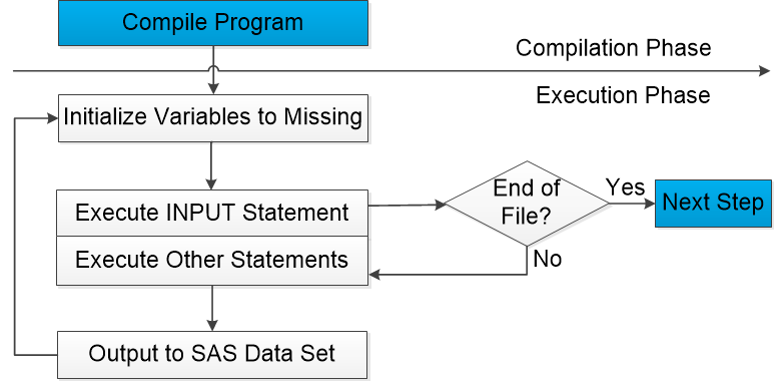
\includegraphics{images/图片1.png}

\hypertarget{ux7f16ux8bd1ux9636ux6bb5}{%
\section{编译阶段}\label{ux7f16ux8bd1ux9636ux6bb5}}

编译阶段会进行语法的检查(keywords缺失或错误,无效的变量名,标点符合的缺失或错误,无效的选项等等),且将SAS语句转换为可执行的机器代码,并创建以下内容:

\begin{enumerate}
\def\labelenumi{\arabic{enumi}.}
\item
  input buffer

  input buffer只会在SAS
  input语句读入数据时才会创建的一个逻辑空间,如果是SAS
  set语句,则会直接创建PDV。可以理解为input
  buffer只有一行的空间,读入数据时,也只能一行一行的读取。

  \begin{longtable}[]{@{}lllllllll@{}}
  \toprule\noalign{}
  \endhead
  \bottomrule\noalign{}
  \endlastfoot
  1 & 2 & 3 & 4 & 5 & 6 & 7 & 8 & \ldots{} \\
  & & & & & & & & \\
  \end{longtable}
\item
  program data vector (PDV)

  PDV也是一个逻辑空间,同样理解为PDV只有一行的空间。会根据运行的SAS程序,创建SAS变量以及两个自动变量\_N\_,\_ERROR\_(自动变量最终不会写入到SAS数据集)。

  \begin{longtable}[]{@{}lllllll@{}}
  \toprule\noalign{}
  \_N\_ & \_ERROR\_ & & & & & \\
  \midrule\noalign{}
  \endhead
  \bottomrule\noalign{}
  \endlastfoot
  & & & & & & \\
  \end{longtable}
\item
  dataset attributesand variable attributes

  在编译阶段就已经确定了SAS数据集与变量的属性(Proc contents
  的输出内容:数据集的名称,观测数,变量数,变量名称,变量属性等等)。
\end{enumerate}

\hypertarget{ux6267ux884cux9636ux6bb5}{%
\section{执行阶段}\label{ux6267ux884cux9636ux6bb5}}

在编译阶段结束时,SAS数据集中是没有观测的。还没有开始执行阶段。执行阶段其实是多次迭代的过程,对数据一行一行的执行。

\begin{enumerate}
\def\labelenumi{\arabic{enumi}.}
\item
  初始化变量(假设读入的数据集有Var1,Var2,Var3三个变量,其中Var3是数值型变量,初始化为.),将变量设置为缺失值(除了自动变量)。

  \begin{longtable}[]{@{}lllll@{}}
  \toprule\noalign{}
  \endhead
  \bottomrule\noalign{}
  \endlastfoot
  \_N\_ & \_ERROR\_ & Var1 & Var2 & Var3 \\
  1 & 0 & & & . \\
  \end{longtable}
\item
  input
  buffer存储第一行记录(仅针对input读入数据,否则跳过),这里还涉及指针(该指针不同于其他语言,是一种虚指),使用指针确当每一个变量的开始与结束。

  \begin{longtable}[]{@{}llllllll@{}}
  \toprule\noalign{}
  \endhead
  \bottomrule\noalign{}
  \endlastfoot
  1 & 2 & 3 & 4 & 5 & 6 & 7 & 8 \\
  T & o & m & & M & & 1 & 5 \\
  \end{longtable}
\item
  在PDV中对变量进行赋值,如果涉及运算如Var4=Var3*10,也会进行处理。

  \begin{longtable}[]{@{}lllll@{}}
  \toprule\noalign{}
  \endhead
  \bottomrule\noalign{}
  \endlastfoot
  \_N\_ & \_ERROR\_ & Var1 & Var2 & Var3 \\
  1 & 0 & Tom & M & 15 \\
  \end{longtable}
\item
  Data step遇到run;或者proc
  xxx;等语句表明执行结束时。会将PDV中变量的值写入到SAS数据集中作为一条观测。\_N\_会被赋值为2(逐步迭代+1),并返回到Data
  step的开头。但是,这里需要注意,分为两种情况:

  如果是通过input语句读入raw
  data,则每一次迭代开始时,对变量初始化为缺失值。(如果程序中通过
  RETAIN, SUM, \_TEMPORARY\_ array
  创建的变量,当然也包括自动变量,则不会被初始化为缺失值。)

  \begin{longtable}[]{@{}lllll@{}}
  \toprule\noalign{}
  \endhead
  \bottomrule\noalign{}
  \endlastfoot
  \_N\_ & \_ERROR\_ & Var1 & Var2 & Var3 \\
  2 & 0 & & & . \\
  \end{longtable}

  如果是通过set语句读入SAS数据集,数据集中的变量则只会在最开始的第一次迭代中对变量初始化为缺失值,后面的迭代中会保留上一次的值直到被替换掉。

  \begin{longtable}[]{@{}lllll@{}}
  \toprule\noalign{}
  \endhead
  \bottomrule\noalign{}
  \endlastfoot
  \_N\_ & \_ERROR\_ & Var1 & Var2 & Var3 \\
  2 & 0 & Tom & M & 15 \\
  \end{longtable}
\item
  当没有更多的数据可以读入,或是SAS遇到end-of-file的标记,则结束执行阶段。并打印SAS
  log.
\end{enumerate}

\hypertarget{macro-ux5b8fux5904ux7406-sas-ux8bedux53e5ux673aux5236}{%
\chapter*{Macro 宏处理 SAS
语句机制}\label{macro-ux5b8fux5904ux7406-sas-ux8bedux53e5ux673aux5236}}
\addcontentsline{toc}{chapter}{Macro 宏处理 SAS 语句机制}

\markboth{Macro 宏处理 SAS 语句机制}{Macro 宏处理 SAS 语句机制}

\hypertarget{ux6ca1ux6709macroux7684sasux8bedux53e5ux8fd0ux884cux673aux5236}{%
\section{没有Macro的SAS语句运行机制}\label{ux6ca1ux6709macroux7684sasux8bedux53e5ux8fd0ux884cux673aux5236}}

在了解macro如何处理SAS语句之前,先来了解一下如果没有macro,SAS如何处理这些命令语句。这里需要介绍两个概念:

\begin{itemize}
\item
  input stack,存放输入的SAS语句
\item
  word scanner,从input
  stack中提取token(token分为literal:引号引起来的字符;number:数字;name:不用引号引起来的字符;special:特殊符号)
\end{itemize}

\begin{longtable}[]{@{}
  >{\raggedright\arraybackslash}p{(\columnwidth - 2\tabcolsep) * \real{0.2083}}
  >{\raggedright\arraybackslash}p{(\columnwidth - 2\tabcolsep) * \real{0.4028}}@{}}
\toprule\noalign{}
\begin{minipage}[b]{\linewidth}\raggedright
word scanner
\end{minipage} & \begin{minipage}[b]{\linewidth}\raggedright
input stack
\end{minipage} \\
\midrule\noalign{}
\endhead
\bottomrule\noalign{}
\endlastfoot
& data class(keep=name age);

set sashelp.class;

run; \\
\end{longtable}

从input
stack中scan第一行的SAS语句,一共有8个token(4个name,4个special)。

\begin{Shaded}
\begin{Highlighting}[]
\NormalTok{data class(keep=name age);}
\end{Highlighting}
\end{Shaded}

当word scanner识别到data这个token,会触发Data step编译器,开始data step
编译阶段,编译器会拉取这些tokens,直到识别到该step结束(如这里的run;),开始data
step的执行阶段。

\hypertarget{ux5177ux6709macroux7684sasux8bedux53e5ux8fd0ux884cux673aux5236}{%
\section{具有Macro的SAS语句运行机制}\label{ux5177ux6709macroux7684sasux8bedux53e5ux8fd0ux884cux673aux5236}}

Macro有macro variable 和 macro statement。

针对macro variable有一个symbol
table,用来存储宏变量的对应信息,包括自动宏变量(如系统内置的宏变量)和全局宏变量。

\begin{longtable}[]{@{}
  >{\raggedright\arraybackslash}p{(\columnwidth - 6\tabcolsep) * \real{0.1528}}
  >{\raggedright\arraybackslash}p{(\columnwidth - 6\tabcolsep) * \real{0.2917}}
  >{\raggedright\arraybackslash}p{(\columnwidth - 6\tabcolsep) * \real{0.2500}}
  >{\raggedright\arraybackslash}p{(\columnwidth - 6\tabcolsep) * \real{0.2222}}@{}}
\toprule\noalign{}
\begin{minipage}[b]{\linewidth}\raggedright
compiler
\end{minipage} & \begin{minipage}[b]{\linewidth}\raggedright
input stack
\end{minipage} & \begin{minipage}[b]{\linewidth}\raggedright
macro processor
\end{minipage} & \begin{minipage}[b]{\linewidth}\raggedright
symbol table
\end{minipage} \\
\midrule\noalign{}
\endhead
\bottomrule\noalign{}
\endlastfoot
& \%let text=``aa'';

data class;

set sashelp.class;

text=\&text;

run; & & sysday Monday \\
\end{longtable}

当word scanner识别到\&或\%这两种token,会触发Macro
processor,对第一行的定义宏变量的语句进行处理。

\begin{Shaded}
\begin{Highlighting}[]
\NormalTok{\%let text="aa";}
\end{Highlighting}
\end{Shaded}

\begin{longtable}[]{@{}
  >{\raggedright\arraybackslash}p{(\columnwidth - 6\tabcolsep) * \real{0.1528}}
  >{\raggedright\arraybackslash}p{(\columnwidth - 6\tabcolsep) * \real{0.2917}}
  >{\raggedright\arraybackslash}p{(\columnwidth - 6\tabcolsep) * \real{0.2500}}
  >{\raggedright\arraybackslash}p{(\columnwidth - 6\tabcolsep) * \real{0.2222}}@{}}
\toprule\noalign{}
\begin{minipage}[b]{\linewidth}\raggedright
compiler
\end{minipage} & \begin{minipage}[b]{\linewidth}\raggedright
input stack
\end{minipage} & \begin{minipage}[b]{\linewidth}\raggedright
macro processor
\end{minipage} & \begin{minipage}[b]{\linewidth}\raggedright
symbol table
\end{minipage} \\
\midrule\noalign{}
\endhead
\bottomrule\noalign{}
\endlastfoot
& data class;

set sashelp.class;

text=\&text;

run; & & sysday Monday

text ``aa'' \\
\end{longtable}

在macro processor运行的时候,data step是没有动作的,只有当macro
processor处理结束后,word scanner 会继续读取SAS语句。而后识别到data
class;中data这个token,会触发data step编译器。

\begin{Shaded}
\begin{Highlighting}[]
\NormalTok{data class; }
\end{Highlighting}
\end{Shaded}

\begin{longtable}[]{@{}
  >{\raggedright\arraybackslash}p{(\columnwidth - 6\tabcolsep) * \real{0.1944}}
  >{\raggedright\arraybackslash}p{(\columnwidth - 6\tabcolsep) * \real{0.2917}}
  >{\raggedright\arraybackslash}p{(\columnwidth - 6\tabcolsep) * \real{0.2500}}
  >{\raggedright\arraybackslash}p{(\columnwidth - 6\tabcolsep) * \real{0.2222}}@{}}
\toprule\noalign{}
\begin{minipage}[b]{\linewidth}\raggedright
compiler
\end{minipage} & \begin{minipage}[b]{\linewidth}\raggedright
input stack
\end{minipage} & \begin{minipage}[b]{\linewidth}\raggedright
macro processor
\end{minipage} & \begin{minipage}[b]{\linewidth}\raggedright
symbol table
\end{minipage} \\
\midrule\noalign{}
\endhead
\bottomrule\noalign{}
\endlastfoot
data class; & set sashelp.class;

text=\&text;

run; & & sysday Monday

text ``aa'' \\
\end{longtable}

compiler会继续从input stack拉取tokens。当word
scanner又识别到\&或\%token的时候,再次触发macro
processor,识别到在symbol table中存在该宏变量,并用 symbol
table中的值替换input stack中的macro variable。

\begin{longtable}[]{@{}
  >{\raggedright\arraybackslash}p{(\columnwidth - 8\tabcolsep) * \real{0.2414}}
  >{\raggedright\arraybackslash}p{(\columnwidth - 8\tabcolsep) * \real{0.1724}}
  >{\raggedright\arraybackslash}p{(\columnwidth - 8\tabcolsep) * \real{0.1609}}
  >{\raggedright\arraybackslash}p{(\columnwidth - 8\tabcolsep) * \real{0.2069}}
  >{\raggedright\arraybackslash}p{(\columnwidth - 8\tabcolsep) * \real{0.1839}}@{}}
\toprule\noalign{}
\begin{minipage}[b]{\linewidth}\raggedright
compiler
\end{minipage} & \begin{minipage}[b]{\linewidth}\raggedright
word scanner
\end{minipage} & \begin{minipage}[b]{\linewidth}\raggedright
input stack
\end{minipage} & \begin{minipage}[b]{\linewidth}\raggedright
macro processor
\end{minipage} & \begin{minipage}[b]{\linewidth}\raggedright
symbol table
\end{minipage} \\
\midrule\noalign{}
\endhead
\bottomrule\noalign{}
\endlastfoot
data class;

set sashelp.class; & text= & ``aa'';

run; & & sysday Monday

text ``aa'' \\
\end{longtable}

而后compiler继续拉取tokens,当word
scanner识别\&或\%token时,继续触发macro
processor,如上述操作,直到识别到该step结束(如这里的run;),开始data
step的执行阶段。

\part{Introduction}

This is a book created from markdown and executable code.

See Knuth (1984) for additional discussion of literate programming.

\hypertarget{introduction-1}{%
\chapter{Introduction}\label{introduction-1}}

This is a book created from markdown and executable code.

See Knuth (1984) for additional discussion of literate programming.

\hypertarget{refs}{}
\begin{CSLReferences}{1}{0}
\leavevmode\vadjust pre{\hypertarget{ref-knuth84}{}}%
Knuth, Donald E. 1984. {``Literate Programming.''} \emph{Comput. J.} 27
(2): 97--111. \url{https://doi.org/10.1093/comjnl/27.2.97}.

\end{CSLReferences}



\end{document}
